\documentclass[11pt, a4paper]{article}
%\usepackage{proj1}
\usepackage{natbib}
\usepackage{fancyhdr}  
\usepackage{subcaption}
\usepackage{caption}
\usepackage{graphicx}
\usepackage{numprint}
\usepackage{multirow}
\linespread{1.25} 
\setlength{\parindent}{0cm}
\graphicspath{{Images/}}
\usepackage{hyperref}
\usepackage{amsmath}
\usepackage{amsfonts}
\usepackage{amssymb}
\usepackage{amsthm}
\usepackage{mathtools}
\usepackage{commath}
\usepackage{bbm}

%\usepackage[sc,osf]{mathpazo}
\usepackage{subcaption}
\usepackage[a4paper, top=1in, left=1.0in, right=1.0in, bottom=1in, includehead, includefoot]{geometry} %Usually have top as 1in

\usepackage{listings}
\usepackage{color} %red, green, blue, yellow, cyan, magenta, black, white
\definecolor{mygreen}{RGB}{28,172,0} % color values Red, Green, Blue
\definecolor{mylilas}{RGB}{170,55,241}


\hypersetup{colorlinks,linkcolor={black},citecolor={blue},urlcolor={black}}
\usepackage{color}
\urlstyle{same}


\theoremstyle{definition}
\newtheorem{definition}{Definition}[section]

%\newcommand{\Sta}{\rho}
\newcommand{\adja}{q_a}
\newcommand{\adjb}{q_b}
\newcommand{\adjaB}{q_{a,\partial \Omega}}
\newcommand{\adjbB}{q_{b,\partial \Omega}}
%\newcommand{\Con}{u}
\newcommand{\ra}{\rho_a}
\newcommand{\rb}{\rho_b}
\newcommand{\w}{\mathbf{w}}
\newcommand{\Stav}{\mathbf{v}}
\newcommand{\Adja}{\mathbf{p}}
\newcommand{\Adjb}{q}
\newcommand{\Adjc}{{p}_{\partial \Sigma}}
\newcommand{\Con}{\mathbf{f}}
\newcommand{\n}{\mathbf{n}}
\newcommand{\h}{\mathbf{h}}
\newcommand{\K}{\mathbf{K}}


\pagenumbering{gobble}
\begin{document}
	\section{Mann Iteration}
Implemented the Mann iteration from the paper. The problem is that $\lambda$ decreases with iterations so it's not really adaptive in the way we'd like it to be.
	
	\begin{figure}[h]
		\centering
		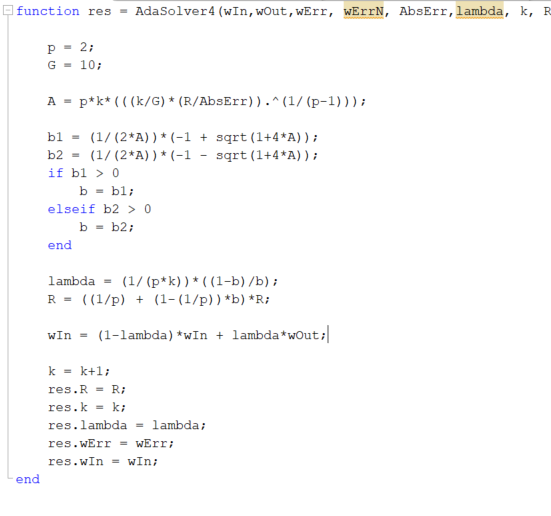
\includegraphics[scale=0.8]{Ada.png}
		\caption{Mann Iteration} 
		\label{F2}
	\end{figure}
	
	
	\section{Optimality Conditions for Two Species}
	We have the following set of forward equations:
	\begin{align*}
	\frac{\partial \ra}{\partial t} =& D_a\nabla^2 \ra - D_a\nabla \cdot(\ra F_a(\w)) + D_a \nabla \cdot (\ra \nabla V_{ext,a}) + D_a\kappa \nabla \cdot \int_\Omega \ra(r) \ra (r') \K_{aa}(r,r')dr' \\
	&+  D_a\tilde{\kappa}\nabla \cdot \int_\Omega \ra(r) \rb (r') \K_{ab}(r,r')dr'\\
	\frac{\partial \rb}{\partial t} =& D_b\nabla^2 \rb - D_b\nabla \cdot(\rb F_b(\w)) + D_b \nabla \cdot (\rb \nabla V_{ext,b}) + D_b\kappa \nabla \cdot \int_\Omega \rb(r) \rb (r') \K_{bb}(r,r')dr' \\
	&+  D_b\tilde{\kappa} \nabla \cdot \int_\Omega \rb(r) \ra (r') \K_{ba}(r,r')dr',
	\end{align*}
	where $D = \frac{1}{\gamma m}$.
	No flux boundary conditions are:
	\begin{align*}
	&\bigg( D_a \nabla \ra - D_a \ra F_a(\w) + D_a \ra \nabla V_{ext,a} + D_a\kappa \int_\Omega \ra(r) \ra (r') \K_{aa}(r,r')dr' \\
	&+  D_a\tilde{\kappa} \int_\Omega \ra(r) \rb (r') \K_{ab}(r,r')dr' \bigg) \cdot \n = 0\\
	&\bigg( D_b \nabla \rb - D_b \rb F_b(\w) + D_b \rb \nabla V_{ext,b} + D_b\kappa \int_\Omega \rb(r) \rb (r')\K_{bb}(r,r')dr' \\
	&+  D_b\tilde{\kappa} \int_\Omega \rb(r) \ra (r') \K_{ba}(r,r')dr' \bigg) \cdot \n = 0
	\end{align*}
	The cost functional is:
	\begin{align*}
	J(\ra,\rb, \w) \coloneqq \frac{1}{2}|| \ra - \widehat{\ra} ||^2_{L_2(\Sigma)} + \frac{\alpha}{2}|| \rb - \widehat {\rb} ||^2_{L_2(\Sigma)} + \frac{\beta}{2}||\w||^2_{L_2(\Sigma)}.
	\end{align*}
	The Lagrangian is then:
	\begin{align*}
	\mathcal{L}(\ra,\rb, \w, \adja, \adjb) =& \frac{1}{2}\int_0^T \int_\Omega ( \ra - \widehat{\ra})^2 dr dt + \frac{\alpha}{2}\int_0^T \int_\Omega ( \rb - \widehat{\rb})^2 dr dt + \frac{\beta}{2}\int_0^T \int_\Omega \w^2 dr dt\\
	& - \int_0^T \int_\Omega \bigg(\frac{\partial \ra}{\partial t} - D_a\nabla^2 \ra + D_a\nabla \cdot(\ra F_a(\w)) - D_a \nabla \cdot (\ra \nabla V_{ext,a})\\
	& - D_a\kappa \nabla \cdot \int_\Omega \ra(r) \ra (r') \K_{aa}(r,r')dr' - D_a\tilde{\kappa} \nabla \cdot \int_\Omega \ra(r) \rb (r') \K_{ab}(r,r')dr\bigg)\adja dr dt \\
	& - \int_0^T \int_\Omega \bigg(
	\frac{\partial \rb}{\partial t} - D_b\nabla^2 \rb + D_b\nabla \cdot(\rb F_b(\w)) - D_b \nabla \cdot (\rb \nabla V_{ext,b}) \\
	&- D_b\kappa \nabla \cdot \int_\Omega \rb(r) \rb (r') \K_{bb}(r,r')dr'
	-  D_b\tilde{\kappa} \nabla \cdot \int_\Omega \rb(r) \ra (r')\K_{ba}(r,r')dr'\bigg) \adjb dr dt\\
	&- \int_0^T \int_{\partial \Omega} \bigg( D_a \nabla \ra - D_a \ra F_a(\w) + D_a \ra \nabla V_{ext,a} + D_a\kappa \int_\Omega \ra(r) \ra (r') \K_{aa}(r,r')dr' \\
	&+  D_a\tilde{\kappa} \int_\Omega \ra(r) \rb (r') \K_{ab}(r,r')dr' \bigg) \cdot \n \adjaB dr dt\\
	& - \int_0^T \int_{\partial \Omega} \bigg( D_b \nabla \rb - D_b \rb F_b(\w) + D_b \rb \nabla V_{ext,b} + D_b\kappa \int_\Omega \rb(r) \rb (r')\K_{bb}(r,r')dr' \\
	&+  D_b\tilde{\kappa} \int_\Omega \rb(r) \ra (r') \K_{ba}(r,r')dr' \bigg) \cdot \n \adjbB dr dt
	\end{align*}
	\section{Adjoint 1}
	Taking the derivative with respect to $\ra$ gives
	\begin{align*}
	\mathcal{L}_{\ra}(\ra,\rb, \w, \adja, \adjb) h &= \int_0^T \int_\Omega ( \ra - \widehat{\ra})h dr dt 
	+ \int_0^T \int_\Omega \bigg(-\frac{\partial h}{\partial t}\adja + D_a\nabla^2 h \adja - D_a\nabla \cdot(h F_a(\w)) \adja\\
	&  + D_a \nabla \cdot (h \nabla V_{ext,a}) \adja + D_a\kappa \nabla \cdot \int_\Omega \adja h(r) \ra (r') \K_{aa}(r,r')dr' \\
	&+ D_a\kappa \nabla \cdot \int_\Omega \adja \ra (r) h (r') \K_{aa}(r,r')dr' + D_a \tilde{\kappa} \nabla \cdot \int_\Omega \adja h(r) \rb (r') \K_{ab} (r,r')dr \bigg)  dr dt \\
	&- \int_0^T \int_{\partial \Omega} \bigg( D_a \nabla h - D_a h F_a(\w) + D_a h \nabla V_{ext,a} + D_a\kappa \int_\Omega h(r) \ra (r') \K_{aa}(r,r')dr' \\
	&+ D_a\kappa \int_\Omega \ra(r) h(r') \K_{aa}(r,r')dr'+  D_a\tilde{\kappa} \int_\Omega h(r) \rb (r') \K_{ab}(r,r')dr' \bigg) \cdot \n \adjaB dr dt\\
	\end{align*}
	And so:
	\begin{align*}
	\mathcal{L}_{\ra}(\ra,\rb, \w, \adja, \adjb) h &= \int_0^T \int_\Omega ( \ra - \widehat{\ra})h dr dt 
	+ \int_0^T \int_\Omega \bigg(\frac{\partial \adja}{\partial t}h + D_a\nabla^2 \adja h + D_a\nabla \adja \cdot(h F_a(\w)) \\
	&  - D_a \nabla \adja \cdot (h \nabla V_{ext,a})  - D_a\kappa \nabla \adja(r) h(r)  \int_\Omega \ra (r') \K_{aa}(r,r')dr' \\
	&- D_a\kappa h (r)\int_\Omega \nabla \adja(r') \ra (r') \K_{aa}(r',r)dr' - D_a \tilde{\kappa} \nabla \adja h(r) \int_\Omega  \rb (r') \K_{ab} (r,r')dr \bigg)  dr dt \\
	&+\int_{ \Omega} \adja(T)h(T) - \adja(0)h(0) dr \\
	&+ \int_0^T \int_{\partial \Omega} D_a \frac{\partial h}{\partial n}\adja - D_a \frac{\partial \adja}{\partial n}h - D_a F_a(\w) h \adja \cdot \n + D_a \nabla V_{ext,a} h \adja \cdot \n dr dt\\
	& + \int_0^T \int_{\partial \Omega} \bigg(D_a \kappa h(r) \adja(r) \int_\Omega \ra(r') \K_{aa}(r,r') \cdot \n dr' \\
	&+  D_a \kappa h(r) \int_{\Omega} \adja(r') \ra(r') \K_{aa}(r'r) \cdot \n dr' 
	+ D_a \tilde{\kappa} \adja(r) h(r) \int_\Omega \rb(r') \K_{ab}(r,r') \cdot \n dr'   \bigg) dr dt\\
	&- \int_0^T \int_{\partial \Omega} \bigg( D_a \nabla h \adjaB- D_a h F_a(\w)\adjaB + D_a h \nabla V_{ext,a}\adjaB\\
	& + D_a\kappa \adjaB(r) h(r)  \int_\Omega \ra (r') \K_{aa}(r,r')dr'
	+ D_a\kappa h(r) \int_\Omega \ra(r') \adjaB(r')  \K_{aa}(r',r)dr'\\
	&+  D_a\tilde{\kappa}\adjaB  h(r)\int_\Omega \rb (r') \K_{ab}(r,r')dr' \bigg) \cdot \n  dr dt\\
	\end{align*}
	Then for $\frac{\partial h}{\partial n} \neq 0$ we get;
	\begin{align*}
	&(D_a \adja - D_a \adjaB) \n = \mathbf 0\\
	&\adja = \adjaB
	\end{align*}
	And all boundary terms cancel so that we get:
	\begin{align*}
	\frac{\partial \adja}{\partial n} = 0 \quad \text{on} \quad \partial \Omega.
	\end{align*}
	And we also get $\adja(T) = 0$.
	
	We get:
	\begin{align*}
	\frac{\partial \adja}{\partial t} = &- D_a\nabla^2\adja - \ra + \widehat{\ra}    - D_a\nabla \adja \cdot F_a(\w) + D_a \nabla \adja \cdot  \nabla V_{ext,a} \\
	&+ D_a\kappa \nabla \adja(r) \int_\Omega \ra (r') \K_{aa}(r,r')dr' + D_a\kappa \int_\Omega \nabla \adja(r') \ra (r') \K_{aa}(r',r)dr' \\
	& + D_a \tilde{\kappa} \nabla \adja \int_\Omega  \rb (r') \K_{ab} (r,r')dr.
	\end{align*}
	\section{Adjoint 2}
	The second adjoint equation is equivalent to the first:
	\begin{align*}
	\frac{\partial \adjb}{\partial t} = &- D_b\nabla^2\adjb - \rb + \widehat{\rb}    - D_b\nabla \adjb \cdot F_b(\w) + D_b \nabla \adjb \cdot  \nabla V_{ext,b} \\
	&+ D_b\kappa \nabla \adjb(r) \int_\Omega \rb (r') \K_{bb}(r,r')dr' + D_b\kappa \int_\Omega \nabla \adjb(r') \rb (r') \K_{bb}(r',r)dr' \\
	& + D_b \tilde{\kappa} \nabla \adjb \int_\Omega  \ra (r') \K_{ba} (r,r')dr.
	\end{align*}
	And the boundary condition is:
	\begin{align*}
	\frac{\partial \adjb}{\partial n} = 0 \quad \text{on} \quad \partial \Omega.
	\end{align*} 
	And we also get $\adjb(T) = 0$.
	
	\section{Gradient Equation}
	The derivative of the Lagrangian with respect to $\w$ is:
	\begin{align*}
	\mathcal{L}_{\w}(\ra,\rb, \w, \adja, \adjb) \h  &= \int_0^T \int_\Omega \bigg( \beta \w \h - D_a \nabla (\ra F_a(\h)) \adja - D_b \nabla (\rb F_b(\h)) \adjb \bigg)dr dt \\
	&+ \int_0^T \int_{\partial \Omega} \bigg( D_a \ra \adjaB F_a(\w)  + D_b \rb \adjbB F_b(\w)     \bigg) \cdot \n dr dt\\
	&= \int_0^T \int_\Omega \bigg( \beta \w \h + D_a \nabla  \adja \cdot (\ra F_a(\h)) 
	+ D_b \nabla \adjb \cdot (\rb F_b(\h)) \bigg)dr dt \\
	&- \int_0^T \int_{\partial \Omega} \bigg( D_a \ra \adjaB F_a(\w)  + D_b \rb \adjbB F_b(\w)     \bigg) \cdot \n dr dt\\
	&+ \int_0^T \int_{\partial \Omega} \bigg(D_a  \adja \ra F_a(\h) \cdot \n + D_b \adjb \rb F_b(\h) \cdot \n \bigg) dr dt.\\
	&= \int_0^T \int_\Omega \bigg( \beta \w \h + D_a \nabla  \adja \cdot (\ra F_a(\h)) 
	+ D_b \nabla \adjb \cdot (\rb F_b(\h)) \bigg)dr dt,
	\end{align*}
	since $\adja = \adjaB$ and $\adjb = \adjbB$ from the adjoint derivation.\\
	This we can only solve if we know about $F_a$ and $F_b$ (I guess technically I can't even write $F(\h)$, maybe only if I assume $F$ to be linear?). Assume $F_a(x) = c_a x$ and $F_b(x) = c_b x$, we get:
	\begin{align*}
	\w  = \frac{1}{\beta}\bigg( D_a c_a  \ra  \nabla \adja + D_b c_b \rb \nabla \adjb \bigg).
	\end{align*}	
	
	
	
	
	
	
	
	
	
	
	
	
	\section*{Optimality Conditions for Two Species}
	We have the following set of forward equations:
	\begin{align*}
	\frac{\partial \ra}{\partial t} =& D_a\nabla^2 \ra - D_a\nabla \cdot(\ra F_a(\w)) + D_a \nabla \cdot (\ra \nabla V_{ext,a}) + D_a\kappa \nabla \cdot \int_\Omega \ra(r) \ra (r') \K_{aa}(r,r')dr' \\
	&+  D_a\tilde{\kappa}\nabla \cdot \int_\Omega \ra(r) \rb (r') \K_{ab}(r,r')dr'\\
	\frac{\partial \rb}{\partial t} =& D_b\nabla^2 \rb - D_b\nabla \cdot(\rb F_b(\w)) + D_b \nabla \cdot (\rb \nabla V_{ext,b}) + D_b\kappa \nabla \cdot \int_\Omega \rb(r) \rb (r') \K_{bb}(r,r')dr' \\
	&+  D_b\tilde{\kappa} \nabla \cdot \int_\Omega \rb(r) \ra (r') \K_{ba}(r,r')dr',
	\end{align*}
	where $D = \frac{1}{\gamma m}$.
	No flux boundary conditions are:
	\begin{align*}
	&\bigg( D_a \nabla \ra - D_a \ra F_a(\w) + D_a \ra \nabla V_{ext,a} + D_a\kappa \int_\Omega \ra(r) \ra (r') \K_{aa}(r,r')dr' \\
	&+  D_a\tilde{\kappa} \int_\Omega \ra(r) \rb (r') \K_{ab}(r,r')dr' \bigg) \cdot \n = 0\\
	&\bigg( D_b \nabla \rb - D_b \rb F_b(\w) + D_b \rb \nabla V_{ext,b} + D_b\kappa \int_\Omega \rb(r) \rb (r')\K_{bb}(r,r')dr' \\
	&+  D_b\tilde{\kappa} \int_\Omega \rb(r) \ra (r') \K_{ba}(r,r')dr' \bigg) \cdot \n = 0
	\end{align*}
	The cost functional is:
	\begin{align*}
	J(\ra,\rb, \w) \coloneqq \frac{1}{2}|| \ra - \widehat{\ra} ||^2_{L_2(\Sigma)} + \frac{\alpha}{2}|| \rb - \widehat {\rb} ||^2_{L_2(\Sigma)} + \frac{\beta}{2}||\w||^2_{L_2(\Sigma)}.
	\end{align*}
	The Lagrangian is then:
	\begin{align*}
	\mathcal{L}(\ra,\rb, \w, \adja, \adjb) =& \frac{1}{2}\int_0^T \int_\Omega ( \ra - \widehat{\ra})^2 dr dt + \frac{\alpha}{2}\int_0^T \int_\Omega ( \rb - \widehat{\rb})^2 dr dt + \frac{\beta}{2}\int_0^T \int_\Omega \w^2 dr dt\\
	& - \int_0^T \int_\Omega \bigg(\frac{\partial \ra}{\partial t} - D_a\nabla^2 \ra + D_a\nabla \cdot(\ra F_a(\w)) - D_a \nabla \cdot (\ra \nabla V_{ext,a})\\
	& - D_a\kappa \nabla \cdot \int_\Omega \ra(r) \ra (r') \K_{aa}(r,r')dr' - D_a\tilde{\kappa} \nabla \cdot \int_\Omega \ra(r) \rb (r') \K_{ab}(r,r')dr\bigg)\adja dr dt \\
	& - \int_0^T \int_\Omega \bigg(
	\frac{\partial \rb}{\partial t} - D_b\nabla^2 \rb + D_b\nabla \cdot(\rb F_b(\w)) - D_b \nabla \cdot (\rb \nabla V_{ext,b}) \\
	&- D_b\kappa \nabla \cdot \int_\Omega \rb(r) \rb (r') \K_{bb}(r,r')dr'
	-  D_b\tilde{\kappa} \nabla \cdot \int_\Omega \rb(r) \ra (r')\K_{ba}(r,r')dr'\bigg) \adjb dr dt\\
	&- \int_0^T \int_{\partial \Omega} \bigg( D_a \nabla \ra - D_a \ra F_a(\w) + D_a \ra \nabla V_{ext,a} + D_a\kappa \int_\Omega \ra(r) \ra (r') \K_{aa}(r,r')dr' \\
	&+  D_a\tilde{\kappa} \int_\Omega \ra(r) \rb (r') \K_{ab}(r,r')dr' \bigg) \cdot \n \adjaB dr dt\\
	& - \int_0^T \int_{\partial \Omega} \bigg( D_b \nabla \rb - D_b \rb F_b(\w) + D_b \rb \nabla V_{ext,b} + D_b\kappa \int_\Omega \rb(r) \rb (r')\K_{bb}(r,r')dr' \\
	&+  D_b\tilde{\kappa} \int_\Omega \rb(r) \ra (r') \K_{ba}(r,r')dr' \bigg) \cdot \n \adjbB dr dt
	\end{align*}
	\section{Adjoint 1}
	Taking the derivative with respect to $\ra$ gives
	\begin{align*}
	\mathcal{L}_{\ra}(\ra,\rb, \w, \adja, \adjb) h &= \int_0^T \int_\Omega ( \ra - \widehat{\ra})h dr dt 
	+ \int_0^T \int_\Omega \bigg(-\frac{\partial h}{\partial t}\adja + D_a\nabla^2 h \adja - D_a\nabla \cdot(h F_a(\w)) \adja\\
	&  + D_a \nabla \cdot (h \nabla V_{ext,a}) \adja + D_a\kappa \nabla \cdot \int_\Omega \adja h(r) \ra (r') \K_{aa}(r,r')dr' \\
	&+ D_a\kappa \nabla \cdot \int_\Omega \adja \ra (r) h (r') \K_{aa}(r,r')dr' + D_a \tilde{\kappa} \nabla \cdot \int_\Omega \adja h(r) \rb (r') \K_{ab} (r,r')dr \bigg)  dr dt \\
	&- \int_0^T \int_{\partial \Omega} \bigg( D_a \nabla h - D_a h F_a(\w) + D_a h \nabla V_{ext,a} + D_a\kappa \int_\Omega h(r) \ra (r') \K_{aa}(r,r')dr' \\
	&+ D_a\kappa \int_\Omega \ra(r) h(r') \K_{aa}(r,r')dr'+  D_a\tilde{\kappa} \int_\Omega h(r) \rb (r') \K_{ab}(r,r')dr' \bigg) \cdot \n \adjaB dr dt\\
	\end{align*}
	And so:
	\begin{align*}
	\mathcal{L}_{\ra}(\ra,\rb, \w, \adja, \adjb) h &= \int_0^T \int_\Omega ( \ra - \widehat{\ra})h dr dt 
	+ \int_0^T \int_\Omega \bigg(\frac{\partial \adja}{\partial t}h + D_a\nabla^2 \adja h + D_a\nabla \adja \cdot(h F_a(\w)) \\
	&  - D_a \nabla \adja \cdot (h \nabla V_{ext,a})  - D_a\kappa \nabla \adja(r) h(r)  \int_\Omega \ra (r') \K_{aa}(r,r')dr' \\
	&- D_a\kappa h (r)\int_\Omega \nabla \adja(r') \ra (r') \K_{aa}(r',r)dr' - D_a \tilde{\kappa} \nabla \adja h(r) \int_\Omega  \rb (r') \K_{ab} (r,r')dr \bigg)  dr dt \\
	&+\int_{ \Omega} \adja(T)h(T) - \adja(0)h(0) dr \\
	&+ \int_0^T \int_{\partial \Omega} D_a \frac{\partial h}{\partial n}\adja - D_a \frac{\partial \adja}{\partial n}h - D_a F_a(\w) h \adja \cdot \n + D_a \nabla V_{ext,a} h \adja \cdot \n dr dt\\
	& + \int_0^T \int_{\partial \Omega} \bigg(D_a \kappa h(r) \adja(r) \int_\Omega \ra(r') \K_{aa}(r,r') \cdot \n dr' \\
	&+  D_a \kappa h(r) \int_{\Omega} \adja(r') \ra(r') \K_{aa}(r'r) \cdot \n dr' 
	+ D_a \tilde{\kappa} \adja(r) h(r) \int_\Omega \rb(r') \K_{ab}(r,r') \cdot \n dr'   \bigg) dr dt\\
	&- \int_0^T \int_{\partial \Omega} \bigg( D_a \nabla h \adjaB- D_a h F_a(\w)\adjaB + D_a h \nabla V_{ext,a}\adjaB\\
	& + D_a\kappa \adjaB(r) h(r)  \int_\Omega \ra (r') \K_{aa}(r,r')dr'
	+ D_a\kappa h(r) \int_\Omega \ra(r') \adjaB(r')  \K_{aa}(r',r)dr'\\
	&+  D_a\tilde{\kappa}\adjaB  h(r)\int_\Omega \rb (r') \K_{ab}(r,r')dr' \bigg) \cdot \n  dr dt\\
	\end{align*}
	Then for $\frac{\partial h}{\partial n} \neq 0$ we get;
	\begin{align*}
	&(D_a \adja - D_a \adjaB) \n = \mathbf 0\\
	&\adja = \adjaB
	\end{align*}
	And all boundary terms cancel so that we get:
	\begin{align*}
	\frac{\partial \adja}{\partial n} = 0 \quad \text{on} \quad \partial \Omega.
	\end{align*}
	And we also get $\adja(T) = 0$.
	
	We get:
	\begin{align*}
	\frac{\partial \adja}{\partial t} = &- D_a\nabla^2\adja - \ra + \widehat{\ra}    - D_a\nabla \adja \cdot F_a(\w) + D_a \nabla \adja \cdot  \nabla V_{ext,a} \\
	&+ D_a\kappa \nabla \adja(r) \int_\Omega \ra (r') \K_{aa}(r,r')dr' + D_a\kappa \int_\Omega \nabla \adja(r') \ra (r') \K_{aa}(r',r)dr' \\
	& + D_a \tilde{\kappa} \nabla \adja \int_\Omega  \rb (r') \K_{ab} (r,r')dr.
	\end{align*}
	\section{Adjoint 2}
	The second adjoint equation is equivalent to the first:
	\begin{align*}
	\frac{\partial \adjb}{\partial t} = &- D_b\nabla^2\adjb - \rb + \widehat{\rb}    - D_b\nabla \adjb \cdot F_b(\w) + D_b \nabla \adjb \cdot  \nabla V_{ext,b} \\
	&+ D_b\kappa \nabla \adjb(r) \int_\Omega \rb (r') \K_{bb}(r,r')dr' + D_b\kappa \int_\Omega \nabla \adjb(r') \rb (r') \K_{bb}(r',r)dr' \\
	& + D_b \tilde{\kappa} \nabla \adjb \int_\Omega  \ra (r') \K_{ba} (r,r')dr.
	\end{align*}
	And the boundary condition is:
	\begin{align*}
	\frac{\partial \adjb}{\partial n} = 0 \quad \text{on} \quad \partial \Omega.
	\end{align*} 
	And we also get $\adjb(T) = 0$.
	
	\section{Gradient Equation}
	The derivative of the Lagrangian with respect to $\w$ is:
	\begin{align*}
	\mathcal{L}_{\w}(\ra,\rb, \w, \adja, \adjb) \h  &= \int_0^T \int_\Omega \bigg( \beta \w \h - D_a \nabla (\ra F_a(\h)) \adja - D_b \nabla (\rb F_b(\h)) \adjb \bigg)dr dt \\
	&+ \int_0^T \int_{\partial \Omega} \bigg( D_a \ra \adjaB F_a(\w)  + D_b \rb \adjbB F_b(\w)     \bigg) \cdot \n dr dt\\
	&= \int_0^T \int_\Omega \bigg( \beta \w \h + D_a \nabla  \adja \cdot (\ra F_a(\h)) 
	+ D_b \nabla \adjb \cdot (\rb F_b(\h)) \bigg)dr dt \\
	&- \int_0^T \int_{\partial \Omega} \bigg( D_a \ra \adjaB F_a(\w)  + D_b \rb \adjbB F_b(\w)     \bigg) \cdot \n dr dt\\
	&+ \int_0^T \int_{\partial \Omega} \bigg(D_a  \adja \ra F_a(\h) \cdot \n + D_b \adjb \rb F_b(\h) \cdot \n \bigg) dr dt.\\
	&= \int_0^T \int_\Omega \bigg( \beta \w \h + D_a \nabla  \adja \cdot (\ra F_a(\h)) 
	+ D_b \nabla \adjb \cdot (\rb F_b(\h)) \bigg)dr dt,
	\end{align*}
	since $\adja = \adjaB$ and $\adjb = \adjbB$ from the adjoint derivation.\\
	This we can only solve if we know about $F_a$ and $F_b$ (I guess technically I can't even write $F(\h)$, maybe only if I assume $F$ to be linear?). Assume $F_a(x) = c_a x$ and $F_b(x) = c_b x$, we get:
	\begin{align*}
	\w  = \frac{1}{\beta}\bigg( D_a c_a  \ra  \nabla \adja + D_b c_b \rb \nabla \adjb \bigg).
	\end{align*}	
	
	
	\section*{Additional Note}
	If we choose the problem to be: 
	\begin{align*}
	&J(\rho, \w) \coloneqq \frac{1}{2}|| \rho - \widehat{\rho} ||^2_{L_2(\Sigma)} + \frac{\beta}{2}||\kappa||^2_{L_2(\Sigma)}\\
	&\text{subject to:}\\
	&\frac{\partial \rho}{\partial t} = \nabla^2 \rho - \nabla \cdot(\rho \w) + D_a \nabla \cdot (\rho \nabla V_{ext}) + \kappa \nabla \cdot \int_\Omega \rho(r) \rho (r') \K(r,r')dr', 
	\end{align*}
	then the only thing that changes in our normal derivation is the gradient equation. This becomes:
	\begin{align*}
	\kappa = - \frac{1}{\beta} \nabla \int_\Omega \rho(r) \rho(r') \K(r,r') dr'.
	\end{align*}
	However, I don't think we can make $\K$ the control (as I thought was possible) because we get:
	\begin{align*}
	\mathcal{L}_{\K}(\rho, \K)h = \int_0^T \int_\Omega \bigg( \beta \K(r,r') \cdot \h(r,r')  + \nabla \int_\Omega \rho(r) \rho(r') \h(r,r') dr' \bigg) dr dt,
	\end{align*}
	for this setup:
	\begin{align*}
	&J(\rho, \w) \coloneqq \frac{1}{2}|| \rho - \widehat{\rho} ||^2_{L_2(\Sigma)} + \frac{\beta}{2}||\K||^2_{L_2(\Sigma)}\\
	&\text{subject to:}\\
	&\frac{\partial \rho}{\partial t} = \nabla^2 \rho - \nabla \cdot(\rho \w) + D_a \nabla \cdot (\rho \nabla V_{ext}) + \kappa \nabla \cdot \int_\Omega \rho(r) \rho (r') \K(r,r')dr'.
	\end{align*}
	
\section*{Other}
- DDFT background flow. I am not sure I am looking for the right thing. Poiseuille 
flow?	
	
	
	
	
	
	
	
\end{document}